\documentclass[9pt]{beamer}

\usepackage{epsfig}
\usepackage{kotex}
\usepackage{graphicx}
\usepackage{latexsym}
\usepackage{amssymb}
\usepackage{amscd}
\usepackage{multirow} 
\usepackage{array}
\usepackage{caption}
\usepackage{rotating}
\usepackage{subfig}
\usepackage{color}
\usepackage{natbib}
\usepackage{lscape}
\usepackage{amsmath, amsthm, amssymb}
\usepackage{epsfig}
\usepackage{graphics}
\usepackage{latexsym}
\usepackage{fancyvrb,enumerate}
\usepackage{mathtools}
\usepackage{verbatim} 
\usepackage{afterpage}
\usepackage[ruled,vlined]{algorithm2e}
\usepackage{hyperref}
\usepackage[flushleft]{threeparttable}
\usepackage{soul}

\DeclarePairedDelimiter\abs{\lvert}{\rvert}
\DeclarePairedDelimiter\norm{\lVert}{\rVert}
\long\def\comment#1{} 

%\newtheorem*{thm}{Theorem}
\newtheorem{thm}{Theorem}[section]
\newtheorem{cor}[thm]{Corollary}
\newtheorem{lem}[thm]{Lemma}
\newcommand{\rb}[1]{\raisebox{-.5em}[0pt]{#1}}
\renewcommand{\baselinestretch}{1.8}
\renewcommand{\mid}{\, | \ }
\newcommand{\eighth}{{\textstyle \frac{1}{8}}}

\def \bD { \boldsymbol{\mathcal{D}} }

\newcommand{\eqdis}{\overset{\mathrm{d}}{=\joinrel=}}
\newcommand{\ba}{\mbox{\boldmath $a$}}
\newcommand{\bd}{\mbox{\boldmath $d$}}
\newcommand{\bff}{\mbox{\boldmath $f$}}
\newcommand{\bg}{\mbox{\boldmath $g$}}
\newcommand{\bl}{\mbox{\boldmath $l$}}
\newcommand{\bu}{\mbox{\boldmath $u$}}
\newcommand{\bv}{\mbox{\boldmath $v$}}
\newcommand{\bx}{\mbox{\boldmath $x$}}
\newcommand{\by}{\mbox{\boldmath $y$}}
\newcommand{\bz}{\mbox{\boldmath $z$}}
\newcommand{\bG}{\mbox{\boldmath $G$}}
\newcommand{\bH}{\mbox{\boldmath $H$}}
\newcommand{\bI}{\mbox{\boldmath $I$}}
\newcommand{\bJ}{\mbox{\boldmath $J$}}
\newcommand{\bL}{\mbox{\boldmath $L$}}
\newcommand{\bQ}{\mbox{\boldmath $Q$}}
\newcommand{\bU}{\mbox{\boldmath $U$}}
\newcommand{\bV}{\mbox{\boldmath $V$}}
\newcommand{\bW}{\mbox{\boldmath $W$}}
\newcommand{\bX}{\mbox{\boldmath $X$}}
\newcommand{\bY}{\mbox{\boldmath $Y$}}
\newcommand{\bZ}{\mbox{\boldmath $Z$}}
\newcommand{\bdm}{\begin{displaymath}}
\newcommand{\edm}{\end{displaymath}}
\newcommand{\bnu}{\mbox{\boldmath $\nu$}}
\newcommand{\btau}{\mbox{\boldmath $\tau$}}
\newcommand{\biota}{\mbox{\boldmath $\iota$}}
\newcommand{\bbeta}{\mbox{\boldmath $\beta$}}
\newcommand{\bomega}{\mbox{\boldmath $\omega$}}
\newcommand{\btheta}{\mbox{\boldmath $\theta$}}
\newcommand{\bepsilon}{\mbox{\boldmath $\epsilon$}}
\newcommand{\bdelta}{\mbox{\boldmath $\delta$}}
\newcommand{\balpha}{\mbox{\boldmath $\alpha$}}
\newcommand{\bxi}{\mbox{\boldmath $\xi$}}
\newcommand{\bgamma}{\mbox{\boldmath $\gamma$}}
\newcommand{\bOmega}{\mbox{\boldmath $\Omega$}}
\newcommand{\bPi}{\mbox{\boldmath $\Pi$}}
\newcommand{\bzeta}{\mbox{\boldmath $\zeta$}}
\newcommand{\bpsi}{\mbox{\boldmath $\psi$}}
\newcommand{\bPsi}{\mbox{\boldmath $\Psi$}}
\newcommand{\blambda}{\mbox{\boldmath $\lambda$}}
\newcommand{\bmu}{\mbox{\boldmath $\mu$}}
\newcommand{\bSigma}{\mbox{\boldmath $\Sigma$}}
\newcommand{\bphi}{\mbox{\boldmath $\phi$}}
\newcommand{\C}{{\rm Cov}}
% \newcommand{\bH}{\bold H}
\newcommand{\bbh}{\bld h}

\usetheme{metropolis}

\usefonttheme[onlymath]{serif}	% 수식 설정!!

\title{Robust principal component analysis for functional snippets}
%\date{\today}
\date[Short Occasion]{April 2, 2021}
\author{Hyunsung Kim}
\institute[Deptartment of Statistics]{Department of Statistics\\ Chung-Ang University}

% A subtitle is optional and this may be deleted
%\subtitle{소제목}

%\author{F.~Author\inst{1} \and S.~Another\inst{2}}
% - Give the names in the same order as the appear in the paper.
% - Use the \inst{?} command only if the authors have different
%   affiliation.

%\institute[Universities of Somewhere and Elsewhere] % (optional, but mostly needed)
%{
%  \inst{1}%
%  Department of Computer Science\\
%  University of Somewhere
%  \and
%  \inst{2}%
%  Department of Theoretical Philosophy\\
%  University of Elsewhere}
% - Use the \inst command only if there are several affiliations.
% - Keep it simple, no one is interested in your street address.

%\date{Conference Name, 2013}
% - Either use conference name or its abbreviation.
% - Not really informative to the audience, more for people (including
%   yourself) who are reading the slides online

\subject{Robust principal component analysis for functional snippets}
% This is only inserted into the PDF information catalog. Can be left
% out. 

% If you have a file called "university-logo-filename.xxx", where xxx
% is a graphic format that can be processed by latex or pdflatex,
% resp., then you can add a logo as follows:

% \pgfdeclareimage[height=0.5cm]{university-logo}{university-logo-filename}
% \logo{\pgfuseimage{university-logo}}

% Delete this, if you do not want the table of contents to pop up at
% the beginning of each subsection:
%\AtBeginSubsection[]
%{
%  \begin{frame}<beamer>{Outline}
%    \tableofcontents[currentsection,currentsubsection]
%  \end{frame}
%}

% Let's get started
\begin{document}

\begin{frame}
  \titlepage
\end{frame}

\begin{frame}{Outline}
	\setbeamertemplate{section in toc}[circle]
%	\setbeamertemplate{subsection in toc}[ball unnumbered]
	\tableofcontents
	% You might wish to add the option [pausesections]
\end{frame}

% allowframebreaks 옵션에서 roman number 안나오게 설정
\setbeamertemplate{frametitle continuation}{}

\section{Introduction}

\begin{frame}[allowframebreaks]{Introduction}
	\begin{itemize}
		\item{
			\textbf{Functional data} is collected in the form of curves or functions in various fields such as meteorology and health science.
		}
		\item{
			 Functional data analysis (FDA) assumes \textbf{smoothness and continuity} on a common domain, but is commonly \textbf{obeserved partially or on a specific subinterval}.
		}
		\item{
			\textbf{Funcional snippet} is an extreme case of partially observed functional data, especially only observed on small intervals.
		}
		\item{
			For its sparsity, there is a major problem on \textbf{a covariance estimation} which is necessary for statistical methods such as a principal component analysis.
		}
	
		\pagebreak
		\item{
			\cite{Yao2005} proposed principal analysis by conditional expectation (PACE) which is used \textbf{a bivariate local smoother} and more recently, \cite{Lin2020} proposed \textbf{a semiparametric method} for a covariance estimation.
		}
		\item{
			But these methods have a disadvantage that easilly \textbf{affected by extreme spikes}, and if the data are contaminated by outlieres, it may give a poor estimation for a functional principal component analysis (FPCA).
		}
		\item{
			To overcome this probelm, we study \textbf{a robust covariance estimation method} based on robust smoothing methods such as \textbf{Huber function} \citep{Huber1964} and \textbf{weighted repeated median (WRM)} \citep{Fried2007}, and combine with a semiparametric method \citep{Lin2020}.
		}
		\item{
			Using the above estimation, we apply FPCA to obtain \textbf{robust FPCs}.
%			Using the robust covariance, we apply FPCA to obtain  the robust result by applying FPCA for a robust covariance estimator.
		}
	\end{itemize}
\end{frame}


\begin{frame}[allowframebreaks]{Functional data}
	\begin{figure}[h]
		\centering
		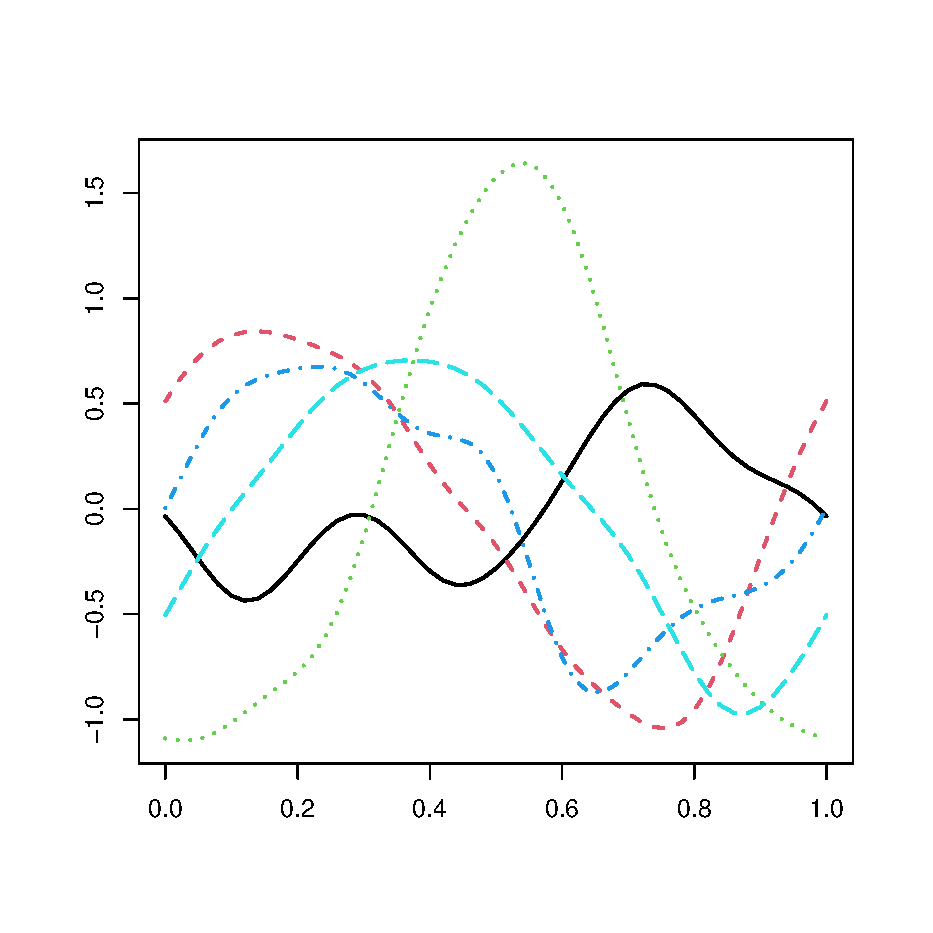
\includegraphics[height=6cm,keepaspectratio=true]{img/funcional_obs.eps}
		\caption{The 5 sample trajectories of completely observed functional data.}
		\label{fig1}
	\end{figure}
\end{frame}

\begin{frame}[allowframebreaks]{Partially observed functional data}
	\begin{figure}[h]
		\centering
		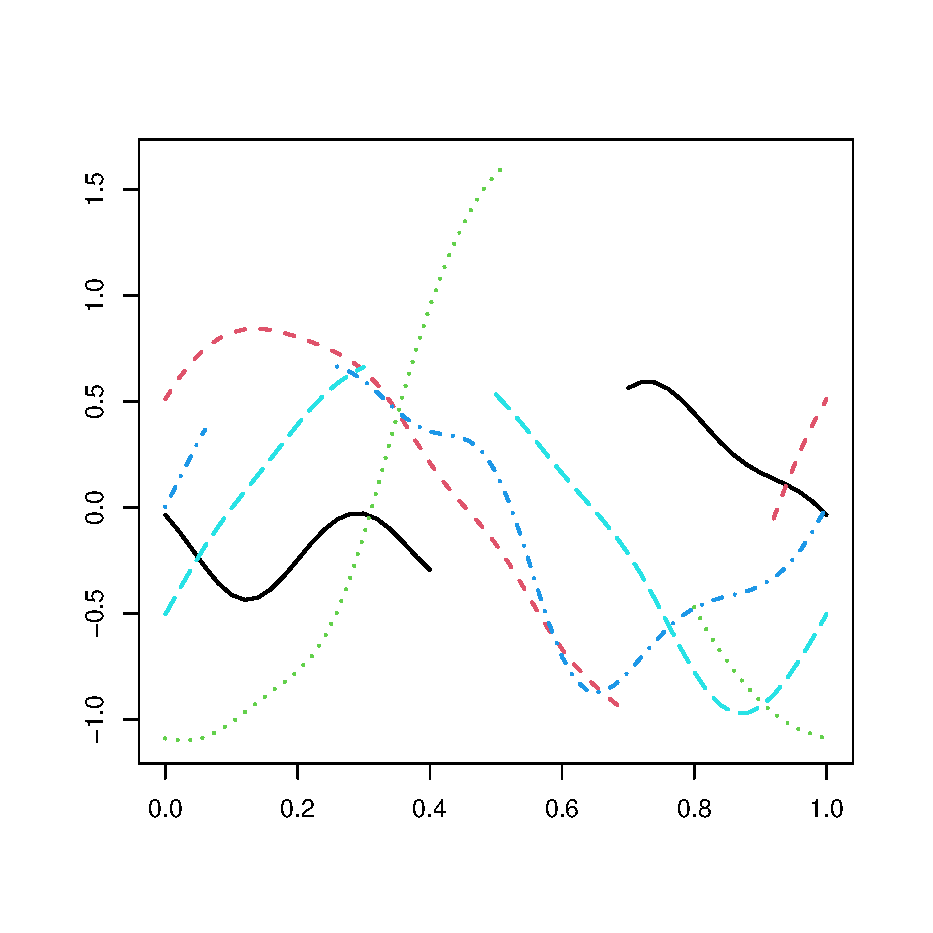
\includegraphics[height=6cm,keepaspectratio=true]{img/partial_obs.eps}
		\caption{The 5 sample trajectories of partially observed functional data.}
		\label{fig2}
	\end{figure}
\end{frame}

\begin{frame}[allowframebreaks]{Functional snippets}
	\begin{figure}[h]
		\centering
		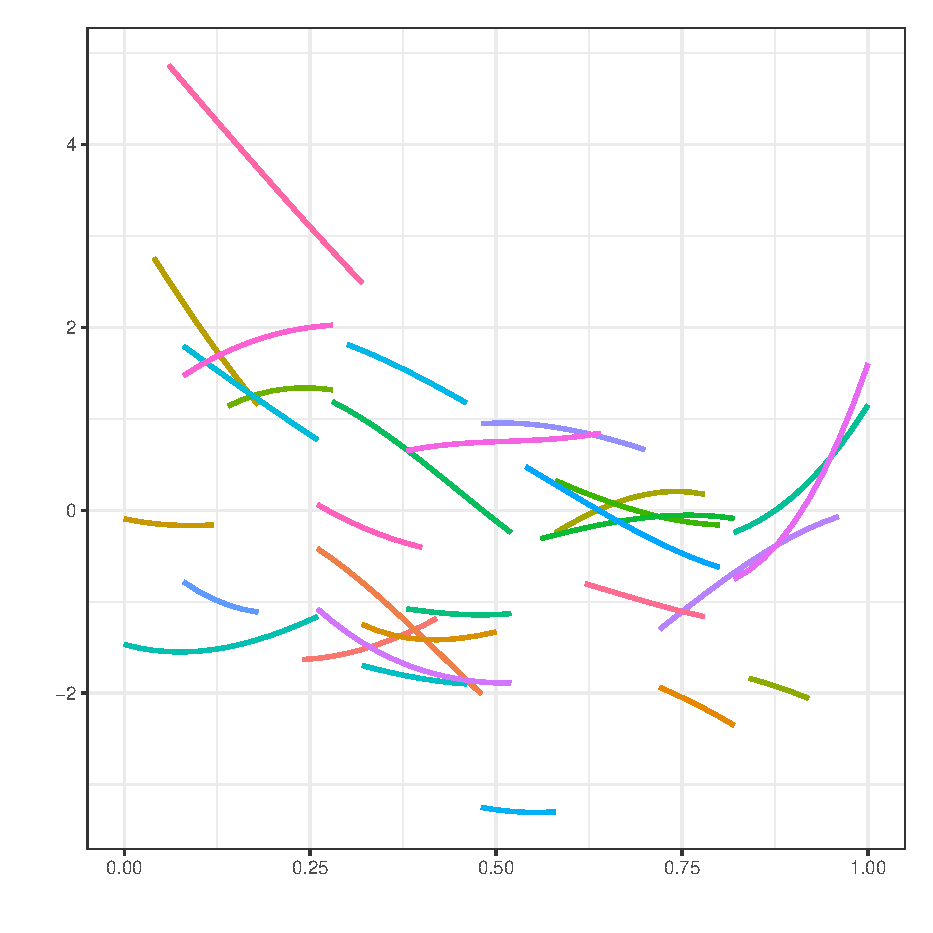
\includegraphics[height=5cm,keepaspectratio=true]{img/fun_snippets.eps}
		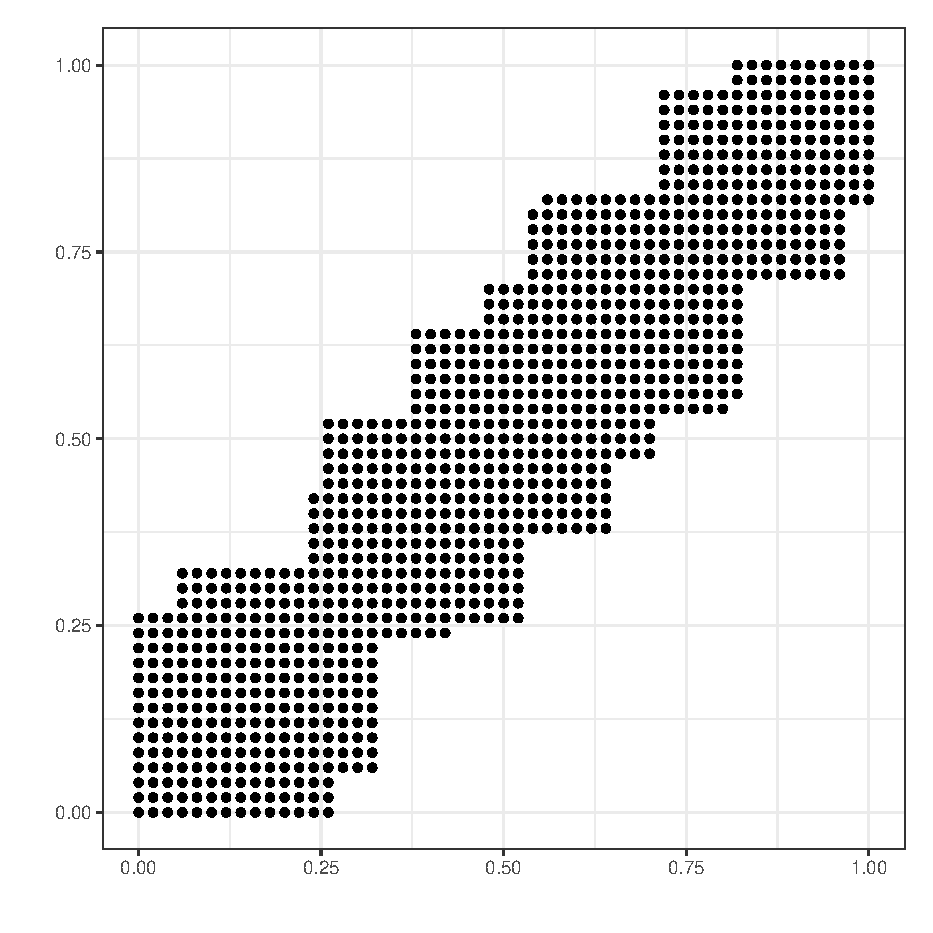
\includegraphics[height=5cm,keepaspectratio=true]{img/fun_snippets_design.eps}
		\caption{The 30 sample trajectories of functional snippets (Left) and its design plot (Right).}
		\label{fig3}
	\end{figure}
\end{frame}

\begin{frame}[allowframebreaks]{Example of functional data}
	\begin{figure}[h]
		\centering
		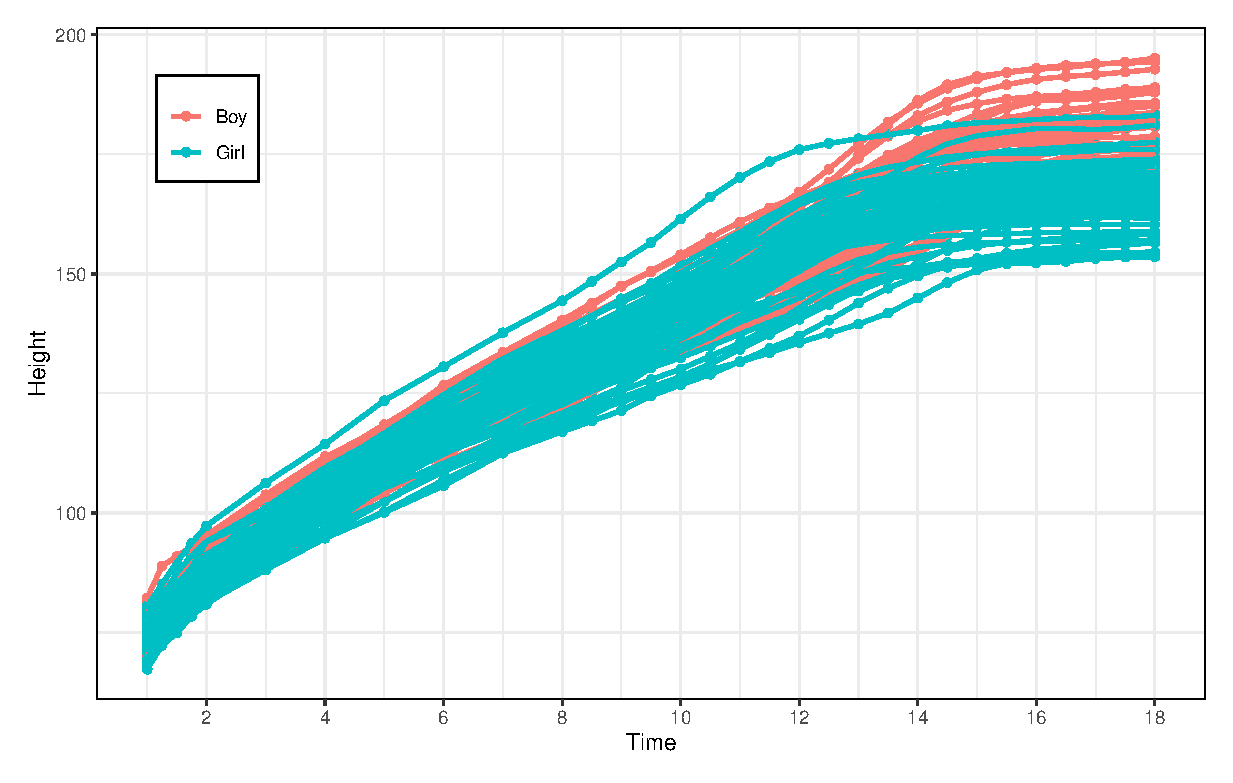
\includegraphics[height=5cm,keepaspectratio=true]{img/growth.eps}
		\caption{Berkely growth data of 93 individuals.}
	\end{figure}
\end{frame}

\begin{frame}[allowframebreaks]{Example of functional snippets}
	\begin{figure}[h]
		\centering
		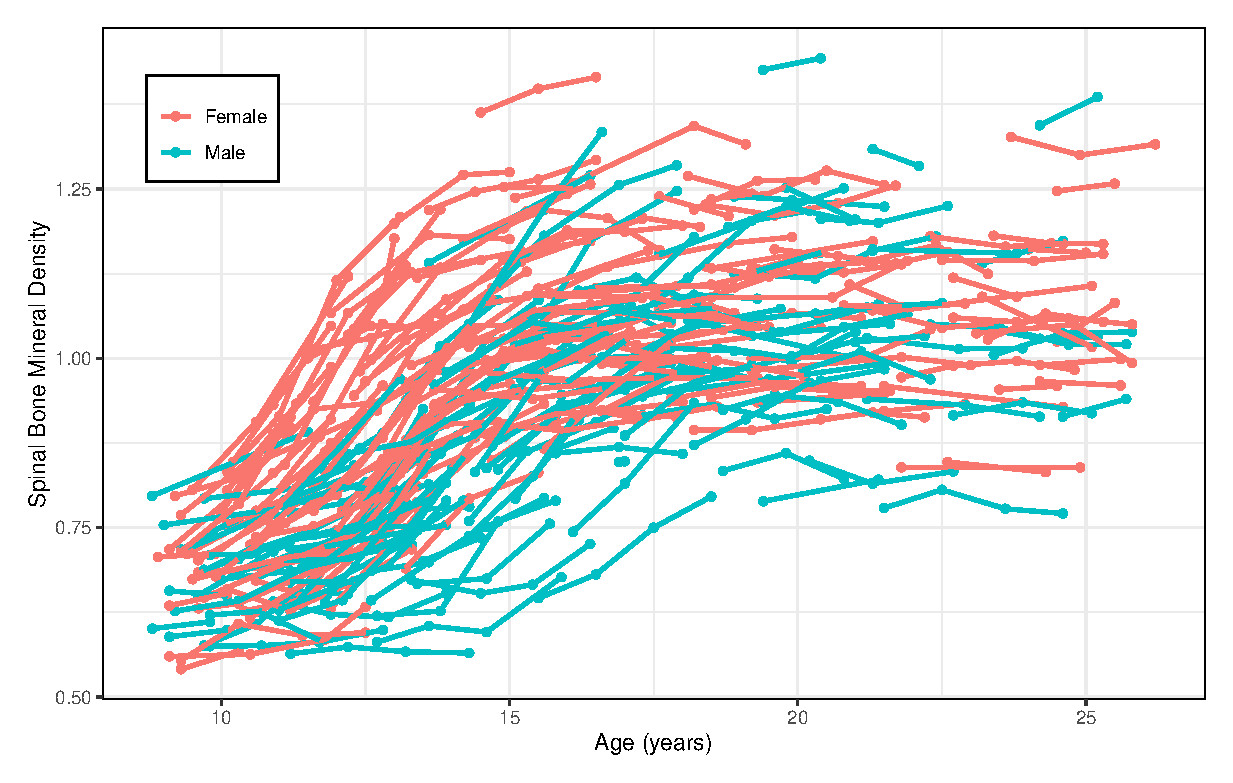
\includegraphics[height=5cm,keepaspectratio=true]{img/spnbmd.eps}
		\caption{Spinal bone mineral density of 280 individuals.}
	\end{figure}
\end{frame}



\section{Method}\label{ch2}

\begin{frame}[allowframebreaks]{Assumptions}
	\begin{itemize}
		\item{
			Let $X$ be a second-order random process defined on an interval $\mathcal{I} \subset \mathbb{R}$ with mean function $\mu(t) = E(X(t))$, and covariance function $C(s,t) = cov(X(s),X(t))$.
		}
		\item{
			Assume the following model,
			$$
			Y_{ij} = X_i(T_{ij}) + \epsilon_{ij}, ~~ \text{for} ~ j=1, \ldots, m_i,~ i=1, \ldots, n,
			$$
			where $X_i$ is observed at time points $T_{i1}, \ldots, T_{im_i}$ and $\epsilon_{ij}$ is the homoscedastic random noise with $E(\epsilon_{ij})=0$ and $E (\epsilon_{ij}^2)= \sigma_0^2$.
		}
	\end{itemize}
\end{frame}


\begin{frame}[allowframebreaks]{Mean function}
	\begin{itemize}
		\item{
			The mean function $\mu(t)$ is estimated by \textbf{a robust local linear smoothing}: 
%			by solving a following minimization criterion:	
			$$
			( \hat b_0 , \hat b_1) = \underset{(b_0,b_1) \in \mathbb{R}^2}{\operatorname{\arg\min}} \sum_{i=1}^n w_i \sum_{j=1}^{m_i} K_{h_\mu} (T_{ij} -t) 
			\rho_\delta  \left\{ \frac {Y_{ij} - b_0 - b_1 (T_{ij} -t) }{s_{\mu}} \right\}
			$$
			where $K_{h_\mu}(\cdot)$ is a kernel function and $h_{\mu}$ is a bandwidth,
			$$ \rho_\delta (x) = \begin{cases} \frac{x^2}{2} , & |x| \leq \delta \\
			\delta \left( |x| - \frac{1}{2} \delta \right) , & |x| > \delta ,
			\end{cases}
			$$
			is the \textbf{Huber function}, a scale parameters $s_\mu$ is estimated by 
			$$ \hat s_{\mu} = 1.4826 \times \text{MAD}\left( \left\{ |Y_{ij} - \hat{b}_0^{*} - \hat{b}_1^{*} (T_{ij} -t)| : i=1,2,\dots,n \right\} \right) , $$
			with $\hat{b}_0^{*}$ and $\hat{b}_1^{*}$ are obtained by least square estimation.
		}
		\item{
			The bandwidth $h_{\mu}$ and $\delta$ in Huber function are selected by 5-fold cross-validation.
		}
	\end{itemize}
\end{frame}


\begin{frame}[allowframebreaks]{Covariance function}
	\begin{itemize}
		\item{
			\cite{Lin2020} proposed \textbf{a semiparametric covariance estimation} which is estimated \textbf{nonparametrically for diagonal parts and parametrically for off-diagonal parts}.
		}
		\item{
			The robust estimation of variance function $\sigma^2_X(t)$ is estimated as
			$$
			\sigma^2_X(t) = \sigma^2_Y(t) - \sigma^2_0 ,
			$$
			where $\sigma^2_Y(t)$ is a variance of the observed data and $\sigma^2_0$ is a noise variance.
		}
		\item{
			By estimating $\sigma^2_Y(t)$ using \textbf{a robust local linear smoothing}, $\sigma^2_X(t)$ can be esimated nonparametrically.
		}
		
	
		\pagebreak
		\item{
			The robust estimation of $\sigma^2_Y(t)$ is obtained from the following minimization criterion:
			\begin{align*}
			( \hat b_0 , \hat b_1) =& \underset{(b_0,b_1) \in \mathbb{R}^2}{\operatorname{\arg\min}} \sum_{i=1}^n w_i \sum_{j=1}^{m_i} K_{h_\sigma} (T_{ij} -t) \\
								    &\times \rho_\delta \left[ \frac{ \{Y_{ij} - \hat \mu(T_{ij})\}^2 -b_0-  b_1 (T_{ij} -t) }{s_{\sigma}} \right], 
			\end{align*}
			where $h_{\sigma}$ is a bandwidth and a scale parameter $s_\sigma$ is estimated by 
			$$ \hat s_{\sigma} = 1.4826 \times \text{MAD}\left( \left\{ |\{Y_{ij} - \hat \mu(T_{ij})\}^2 - \hat{b}_0^{*} - \hat{b}_1^{*} (T_{ij} -t)| : i=1,2,\dots,n \right\} \right) , $$
			with $\hat{b}_0^{*}$ and $\hat{b}_1^{*}$ are obtained by least square estimation.
		}
		\item{
			The bandwidth $h_{\sigma}$ and $\delta$ in Huber function are selected by 5-fold cross-validation.
		}
		
	
		\pagebreak
		\item{
			For off-diagonal parts of the covariance function, we use a \textbf{Mat\'{e}rn correlation} which is a popular \textbf{parametric correlation structure}.
			$$
			r_{\theta}(s,t) = \frac{1}{ \Gamma(\theta_1) 2^{\theta_1 -1} }  \Big( \sqrt{2 \theta_1} \frac{ | s-t | }{\theta_2} \Big)^{\theta_1} B_{\theta_1} \Big( \sqrt{2 \theta_1} \frac{ | s-t | }{\theta_2} \Big) ,~~~ \theta_1 , \theta_2 >0, 
			$$
			where $B_{\theta}(\cdot)$ is the modified Bessel function of the second kind of order $\theta$.
		}
		\item{
			Given the estimate $\hat\sigma^2_X(t)$, the parameter $\theta$ is estimated using the following least squares criterion,
			$$  \underset{\theta}{\operatorname{\arg\min}} \sum_{i=1}^n \frac{1}{ m_i (m_i -1) }\sum_{ 1 \leq j \neq l \leq m_i} \{ \hat \sigma_X (T_{ij} ) \hat \sigma_X (T_{il} )
			r_{\theta}(T_{ij} , T_{il}) - C_{ijl} \}^2,$$
			where $C_{ijl} = \{ Y_{ij} - \hat \mu (T_{ij} ) \} \{ Y_{il} - \hat \mu (T_{il} ) \} $.
		}
		\item{
			Then, the off-diagonal of covariance function can be obtaind as
			$$
			\hat C(s,t) = \hat\sigma_X(s) \hat\sigma_X(t) r_{\hat\theta}(s,t).
			$$
		}
	\end{itemize}
\end{frame}


\begin{frame}[allowframebreaks]{Noise variance estimation}
	\begin{itemize}
		\item{
			\cite{Lin2020} proposed the noise varaince estimation without any other parameters, but if there exists outliers, the estimation is very \textbf{sensitive to the scale of data}.
		}
		\item{
			To obtain an estimation resistant to outliers, we substitute the average term to a robust scale estimator, \textbf{median} as follows:
			\begin{align*}
				\hat{A}_0 &= \text{median} \left\{ \frac{1}{m_i(m_i-1)} \sum_{j \ne l} Y_{ij}^21_{|T_{ij}-T_{il}|<h_0} \right\} \\
				\hat{A}_1 &= \text{median} \left\{ \frac{1}{m_i(m_i-1)} \sum_{j \ne l} Y_{ij} Y_{il} 1_{|T_{ij}-T_{il}|<h_0} \right\} \\
				\hat{B}   &= \text{median} \left\{ \frac{1}{m_i(m_i-1)} \sum_{j \ne l} 1_{|T_{ij}-T_{il}|<h_0} \right\},
			\end{align*}
			where $h_0$ is the bandwidth.
		}
		
		\pagebreak
		\item{
			Then, the noise variance $\sigma_0^2$ can be estimated by
			$$
			\hat\sigma^2_0 = ( \hat{A}_0 - \hat{A}_1 ) / \hat{B}.
			$$
		}
		\item{
			Here, we use the empirical bandwith as 
			$$
			h_0 = 0.29  \hat \xi \lVert \hat\sigma_Y \rVert_2 (n m^2)^{-1/5},
			$$
			where $\hat \xi = \max_{1 \leq i \leq n} \max_{1 \leq j,l \leq m_i} | T_{ij} - T_{il}|$ with $m= n^{-1} \sum_{i=1}^n m_i$.
		}
	\end{itemize}
\end{frame}


\begin{frame}[allowframebreaks]{Parameter selection}
	\begin{itemize}
		\item{
			The optimal $\delta$ in the Huber function is selected by 5-fold CV with the following validation measure,
			\begin{align*}
				\text{CV}(\delta_{\mu}) &= \sum_{k=1}^{\mathcal{K}} \sum_{i \in \mathcal{P}_k} \sum_{j=1}^{m_i} \left| Y_{ij} - \hat{\mu}_{h_{\mu},-k}(T_{ij}) \right| \\
				\text{CV}(\delta_{\sigma}) &= \sum_{k=1}^{\mathcal{K}} \sum_{i \in \mathcal{P}_k} \sum_{j=1}^{m_i} \left| \{ Y_{ij} - \hat{\mu}(T_{ij}) \}^2 - \hat{\sigma}_X^2(T_{ij}) \right|,
			\end{align*}
			where $\mathcal{P}_k$ is a $k$th fold from the training set, $k=1,\dots,5$.
		}
		\item{
			The optimal bandwidth $h_{\mu}$ and $h_{\sigma}$ are selected by 5-fold CV with the following validation measure,
			\begin{align*}
				\text{CV}(h_{\mu}) &= \sum_{k=1}^{\mathcal{K}} \sum_{i \in \mathcal{P}_k} \sum_{j=1}^{m_i} \rho_{\delta_{\mu}} \left\{ Y_{ij} - \hat{\mu}_{h_{\mu},-k}(T_{ij}) \right\} \\
				\text{CV}(h_{\sigma}) &= \sum_{k=1}^{\mathcal{K}} \sum_{i \in \mathcal{P}_k} \sum_{j=1}^{m_i} \rho_{\delta_{\sigma}} \left[ \{ Y_{ij} - \hat{\mu}(T_{ij}) \}^2 - \hat{\sigma}_{X;h_{\sigma}, -k}^2(T_{ij}) \right].
			\end{align*}
		}
	\end{itemize}
\end{frame}



\section{Simulation}

\begin{frame}[allowframebreaks]{Simulation settings}
	\begin{itemize}
		\item{
			$X_i (t_{ij}), ~ i=1, \ldots, 100$ are normally distributed with mean zero and covariance $cov\{ X_{i} (t_{ij}) ) , X_{i} (t_{ik}) \}= C (t_{ij}, t_{ik})$ which is defined as
			$$ C(s,t) = \sum_{i=1}^4 0.5^{i-1} \phi_i (t) \phi_i (s), $$
			where $\phi_1(t) =1 , ~\phi_2(t) = (2t-1) \sqrt{3} , ~ \phi_3(t) = (6t^2-6t+1) \sqrt{5}$, and $\phi_4(t) = (20 t^3 - 30 t^2 +12 t -1) \sqrt{7}$.
		}
		\item{
			The observed time points are $t_{ij} \in \mathcal{I}_{D,i}$, where $  \mathcal{I}_{D,i} = \mathcal{I}_i \cup \mathcal{I}_D$. 
			Here, $ \mathcal{I}_i = [A_i, B_i]$ where $A_i = \max (0, M_i - l_i/2)$ and $B_i = \min (1, M_i + l_i/2)$ with $l_i \sim U(a_l , b_l)$ 
			and $M_i \sim U(\frac{a_l}{2} , 1- \frac{a_l}{2})$ for some constants $0<a_l < b_l<1$.
		}
		\item{
			In this simulation, we took $a_l=0.1, ~b_l = 0,3$.
			$ \mathcal{I}_D = \{ t_1 =0 < t_2 < \cdots < t_{50}=1\}$, which are equispaced points.  
		}
	
		\pagebreak
		\item{
			For outliers, we assume the following models: 
			\begin{align}
			X(t) &= \sigma(t)\epsilon(t) \label{outlier1} \\
			X(t) &= \zeta(t) \label{outlier23}
			\end{align}
		}
		\item{
			For outlier 1, we consider the model \eqref{outlier1} with $\epsilon(t)$ and $\sigma(t)$ are generated from $t_3$, $N(2,10^2)$, respectively.
		}
		\item{
			Outlier 2 and 3 are generated from the model \eqref{outlier23} with Cauchy processes with different scales.
		}
		\item{
			For the scale parameter in Cauchy, we consider white noise error for outlier 2, and exponential spatial correlations with unit variance for outlier 3.
		}
		\item{
			The exponential spatial correlation is $\text{Cor}(\zeta(t_1), \zeta(t_2)) = \exp(-|t_1-t_2|/d)$, and in this study, the range parameter $d=0.3$ is used.
		}
	\end{itemize}


    \pagebreak
	\vspace*{0pt}
	\begin{figure}[h]
		\centering
		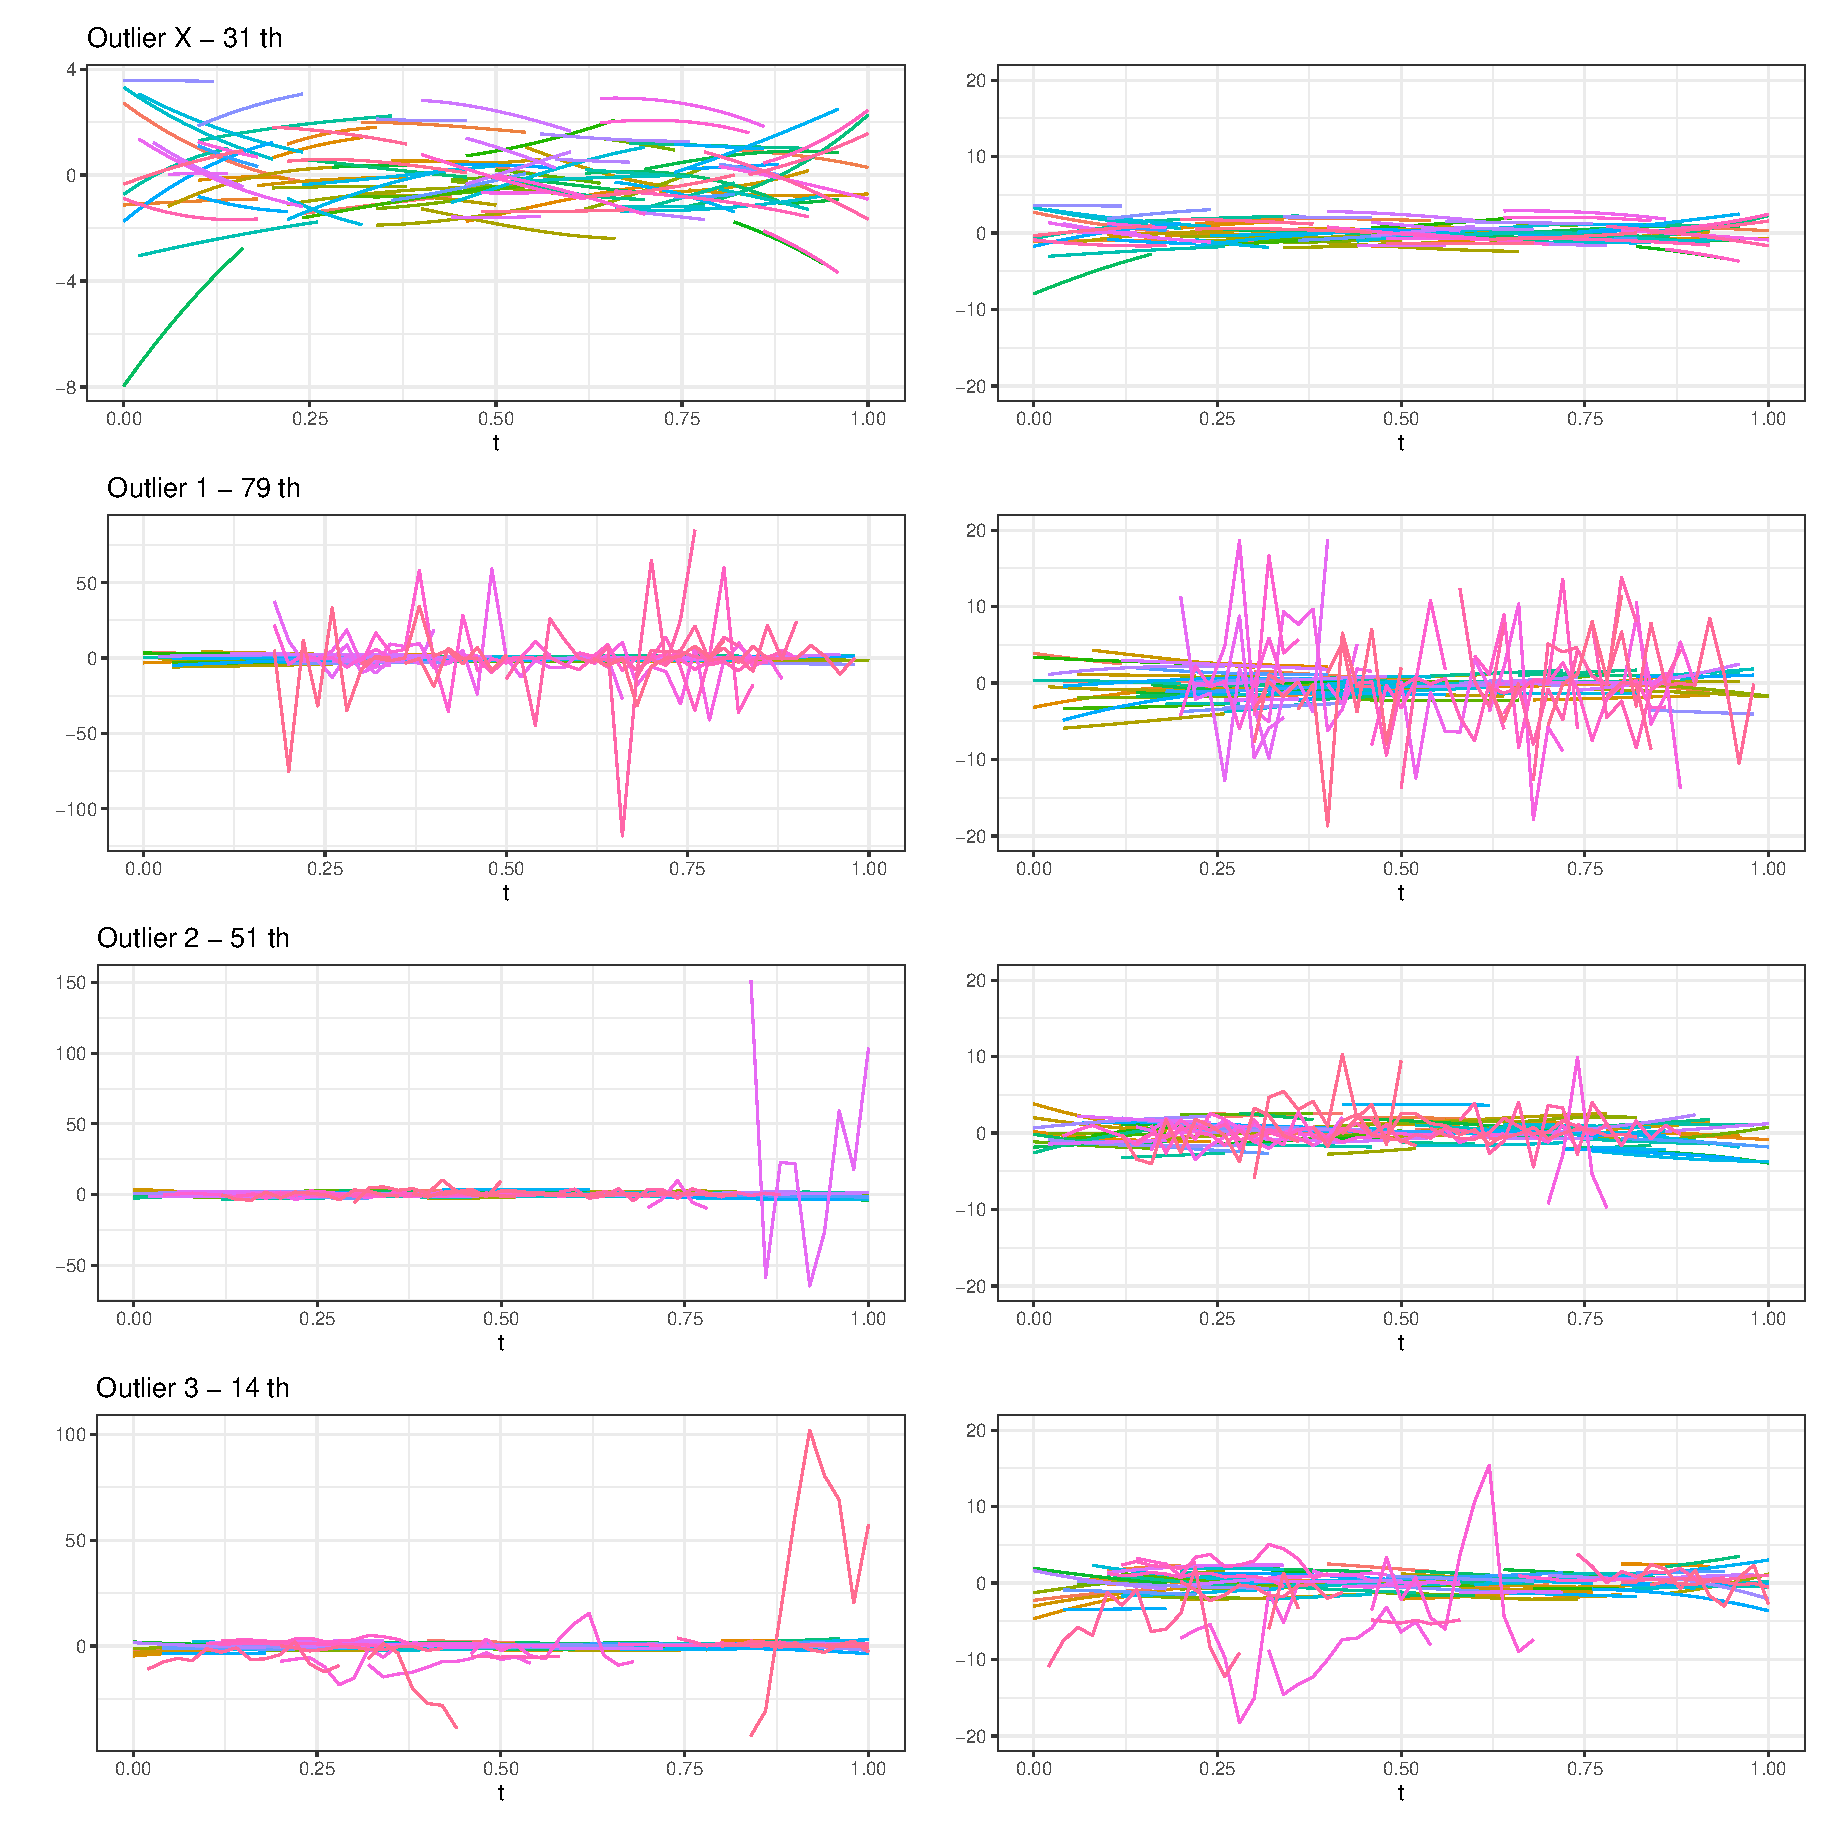
\includegraphics[height=5.5cm,keepaspectratio=true]{img/samp_traj.eps}
		\caption{Sample trajectories for a randomly selected simulation data. It shows generated curves on whole (Left) and limited y-axes (Right).}
		\label{fig4}
	\end{figure}
\end{frame}

\begin{frame}[allowframebreaks]{Performance measures}
	\begin{itemize}
		\item{
			\textbf{Variance estimation}
			$$
			\text{RMISE} = \sqrt{ \frac{1}{N} \sum_{i=1}^N \int_{\mathcal{T}} |\hat{\sigma}^2_X(t) - \sigma^2_X(t)|^2 dt} 
			$$
		}
		\item{
			\textbf{Covariance estimation}
			$$
			\text{RMISE} = \sqrt{ \frac{1}{N} \sum_{i=1}^N \int_{\mathcal{T}}\int_{\mathcal{T}} |\hat{C}(s,t) - C(s,t)|^2 dsdt}
			$$
		}
		
		\pagebreak
		\item{
			\textbf{Intrapolation}
			$$
			\text{RMISE} = \sqrt{ \frac{1}{N} \sum_{i=1}^N \int_{\mathcal{D}_0} |\hat{C}(s,t) - C(s,t)|^2},
			$$
			where $\mathcal{D}_0 := \cup_{i=1}^n ( \mathcal{I}_i \times \mathcal{I}_i )$, where the computation of standard covariance estimators from the raw data is possible.
		}
		\item{
			\textbf{Extrapolation}
			$$
			\text{RMISE} = \sqrt{ \frac{1}{N} \sum_{i=1}^N \int_{\mathcal{S}_0 \backslash \mathcal{D}_0} |\hat{C}(s,t) - C(s,t)|^2},
			$$
			where $\mathcal{S}_0 :=  \mathcal{I} \times \mathcal{I}$, where extrapolation is needed.
		}
	\end{itemize}
	
\end{frame}


\begin{frame}[allowframebreaks]{Estimated variance trajectories}
	\begin{figure}[h]
		\centering
		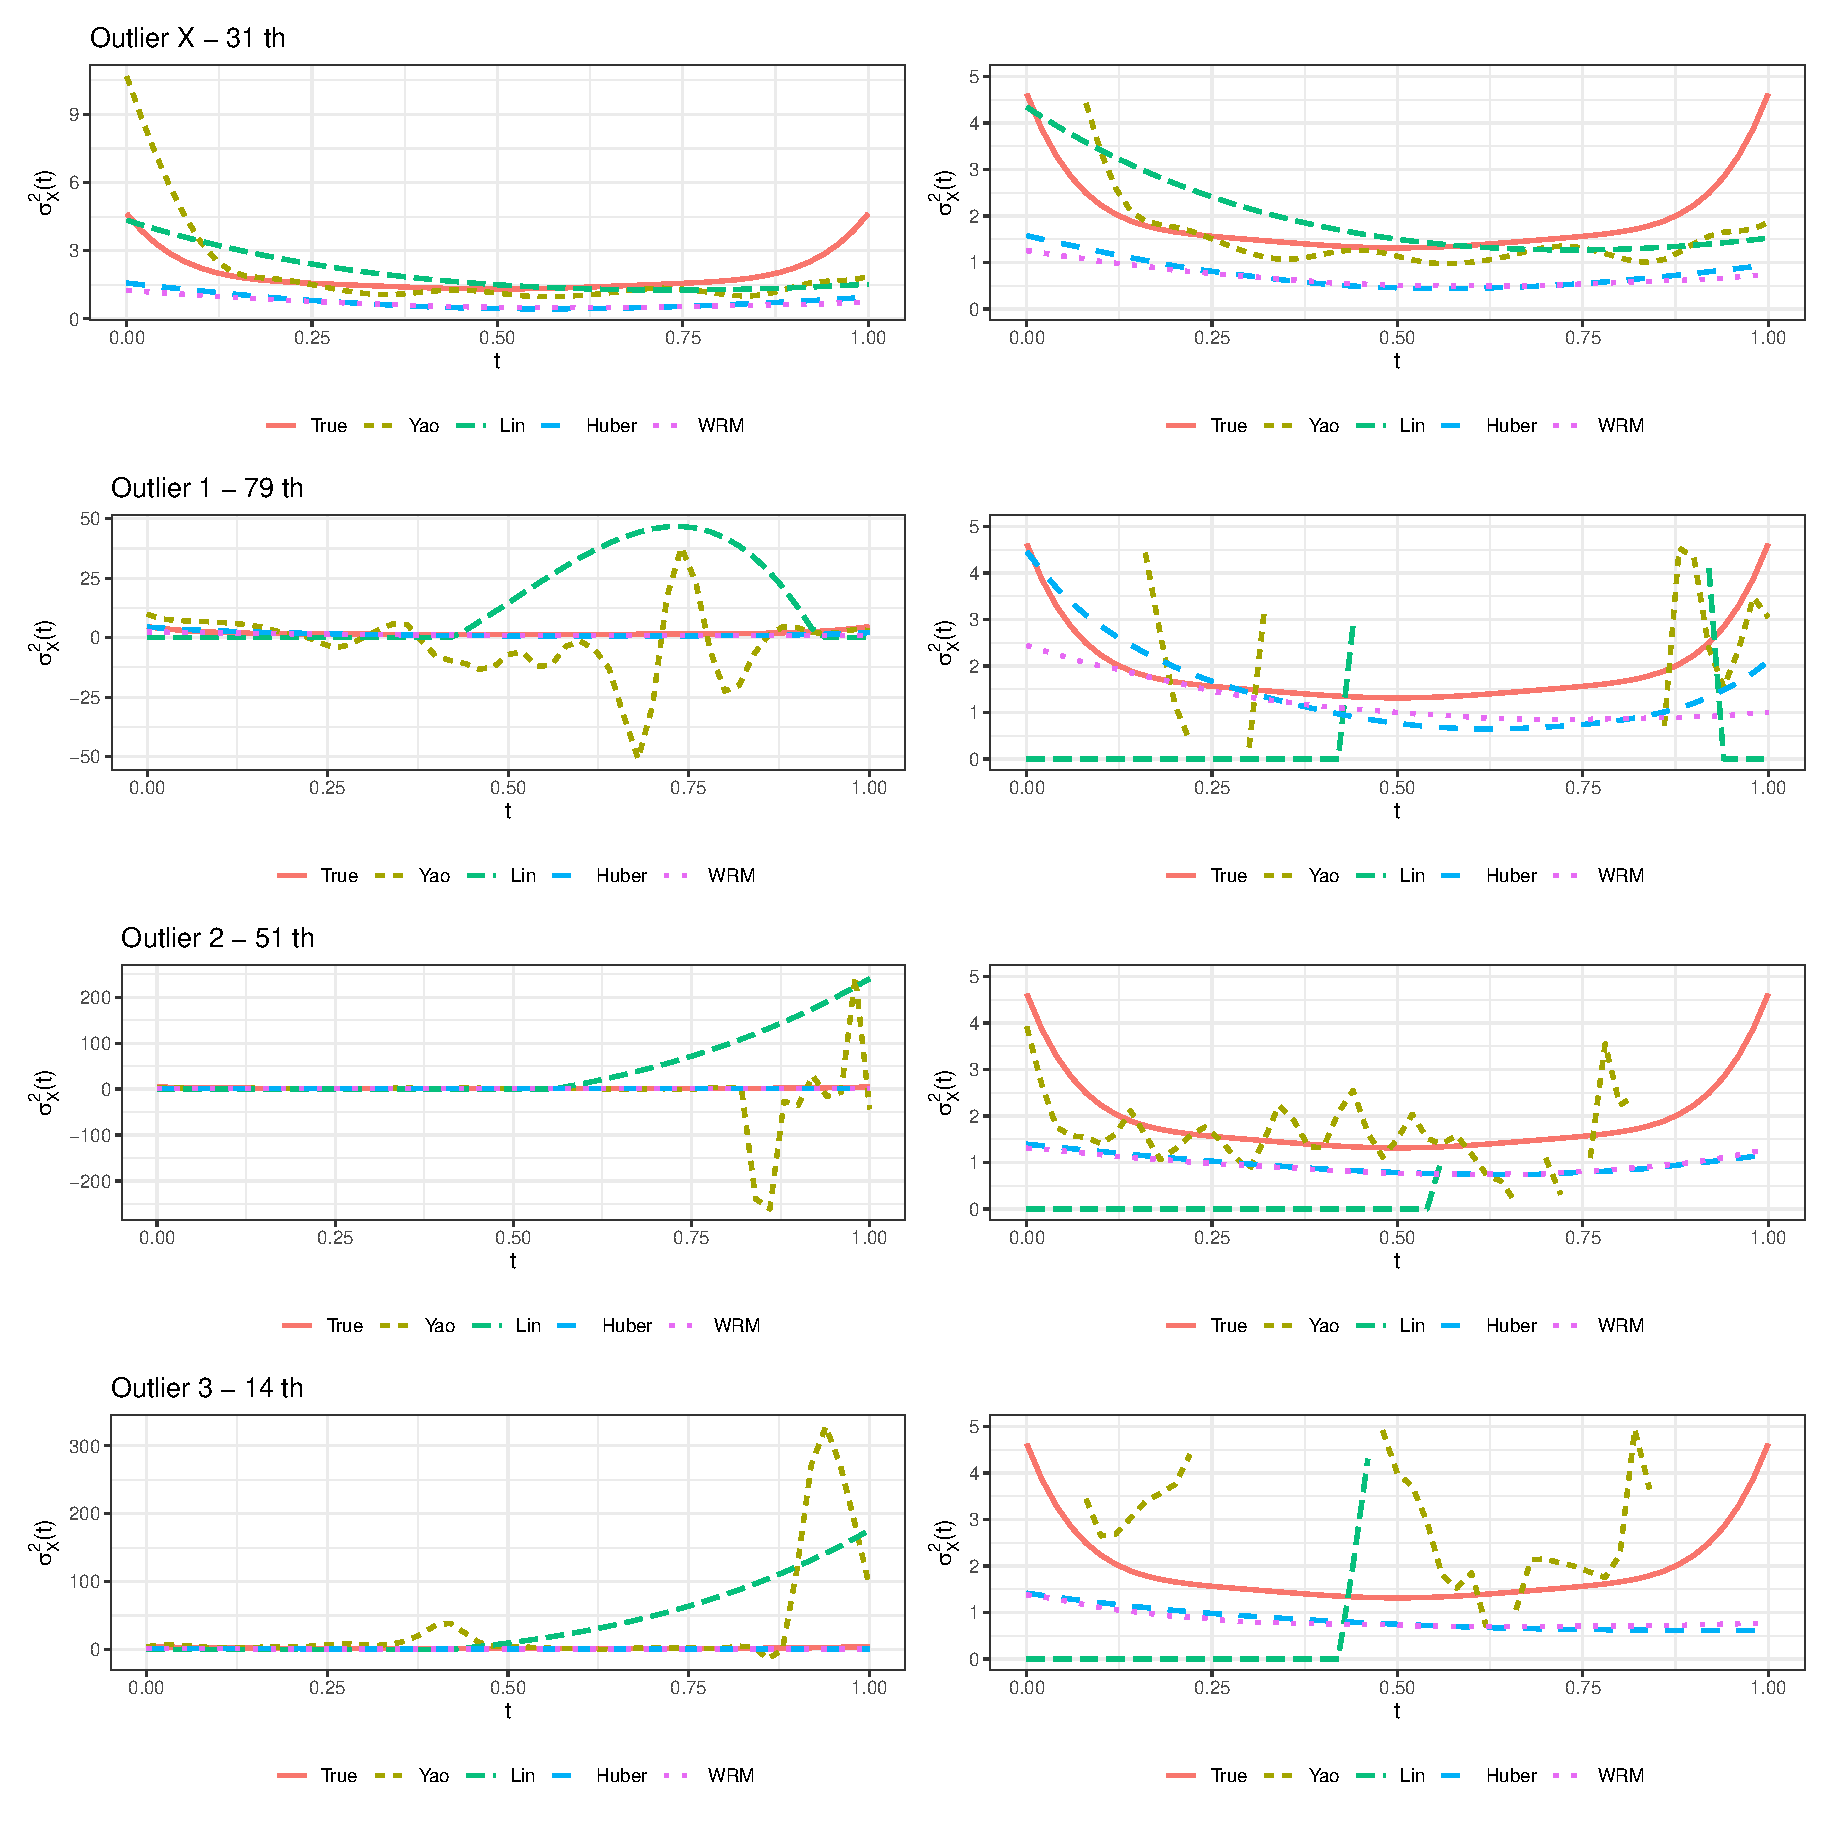
\includegraphics[height=6cm,keepaspectratio=true]{img/var_traj.eps}
		\caption{Estimated variance trajectories for a randomly selected simulation data.}
		\label{fig5}
	\end{figure}
\end{frame}


\begin{frame}[allowframebreaks]{Estimated covariance surfaces}
	\begin{figure}[h]
		\centering
		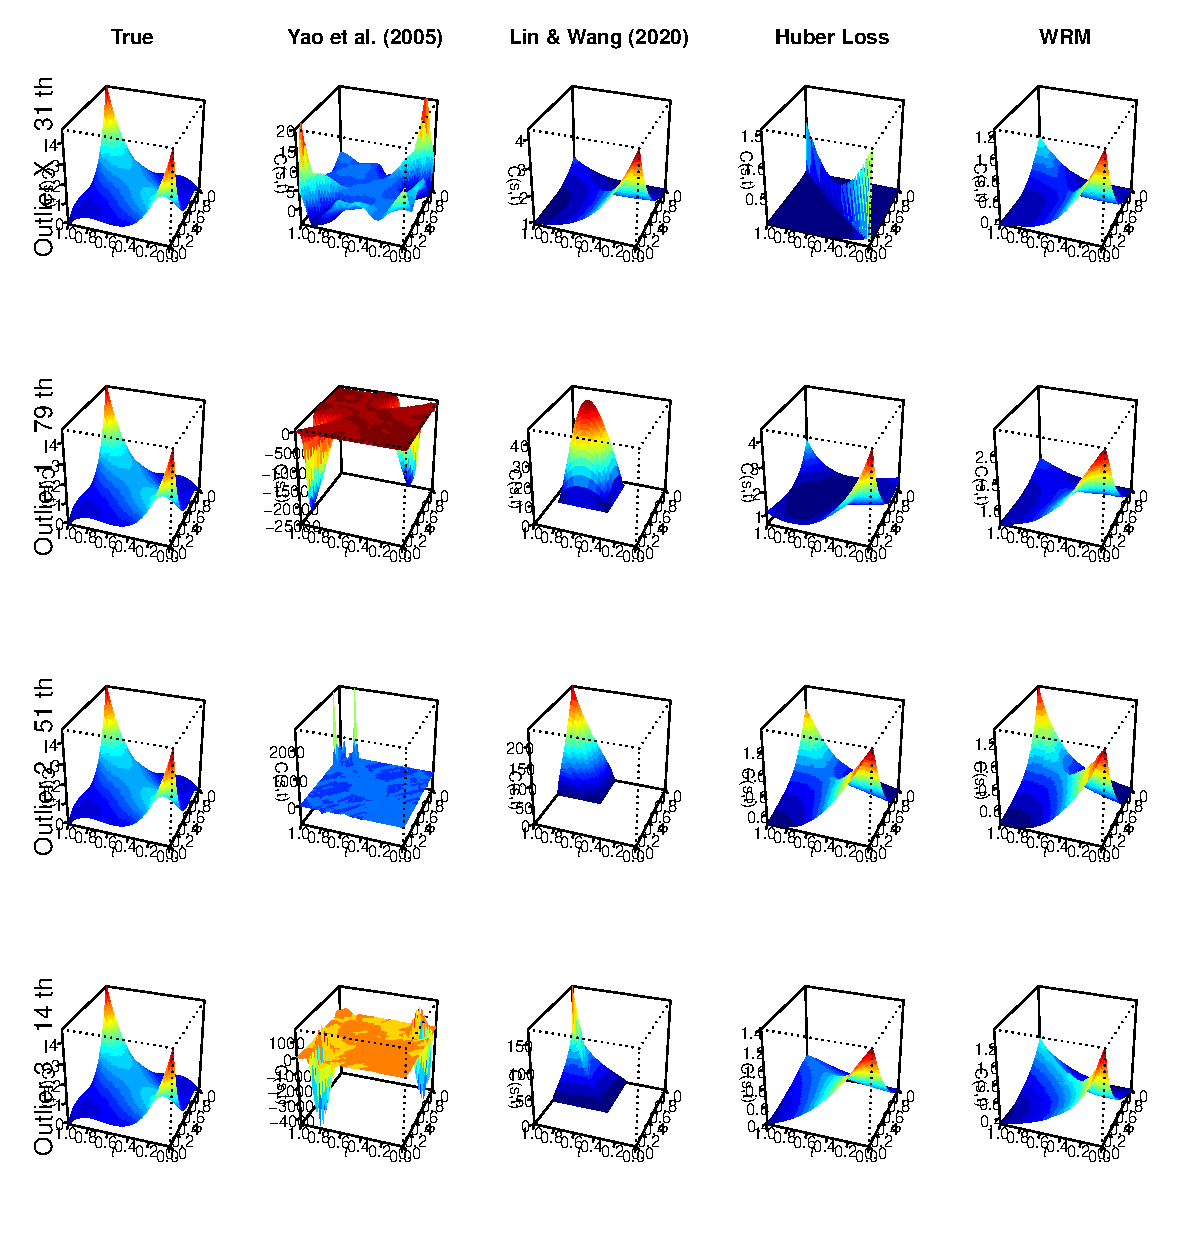
\includegraphics[height=6cm,keepaspectratio=true]{img/cov_surf.eps}
		\caption{True and estimated covariance surfaces for a randomly selected simulation data.}
		\label{fig6}
	\end{figure}
\end{frame}

\begin{frame}[allowframebreaks]{Estimated eigenfunctions}
	\begin{figure}[h]
		\centering
		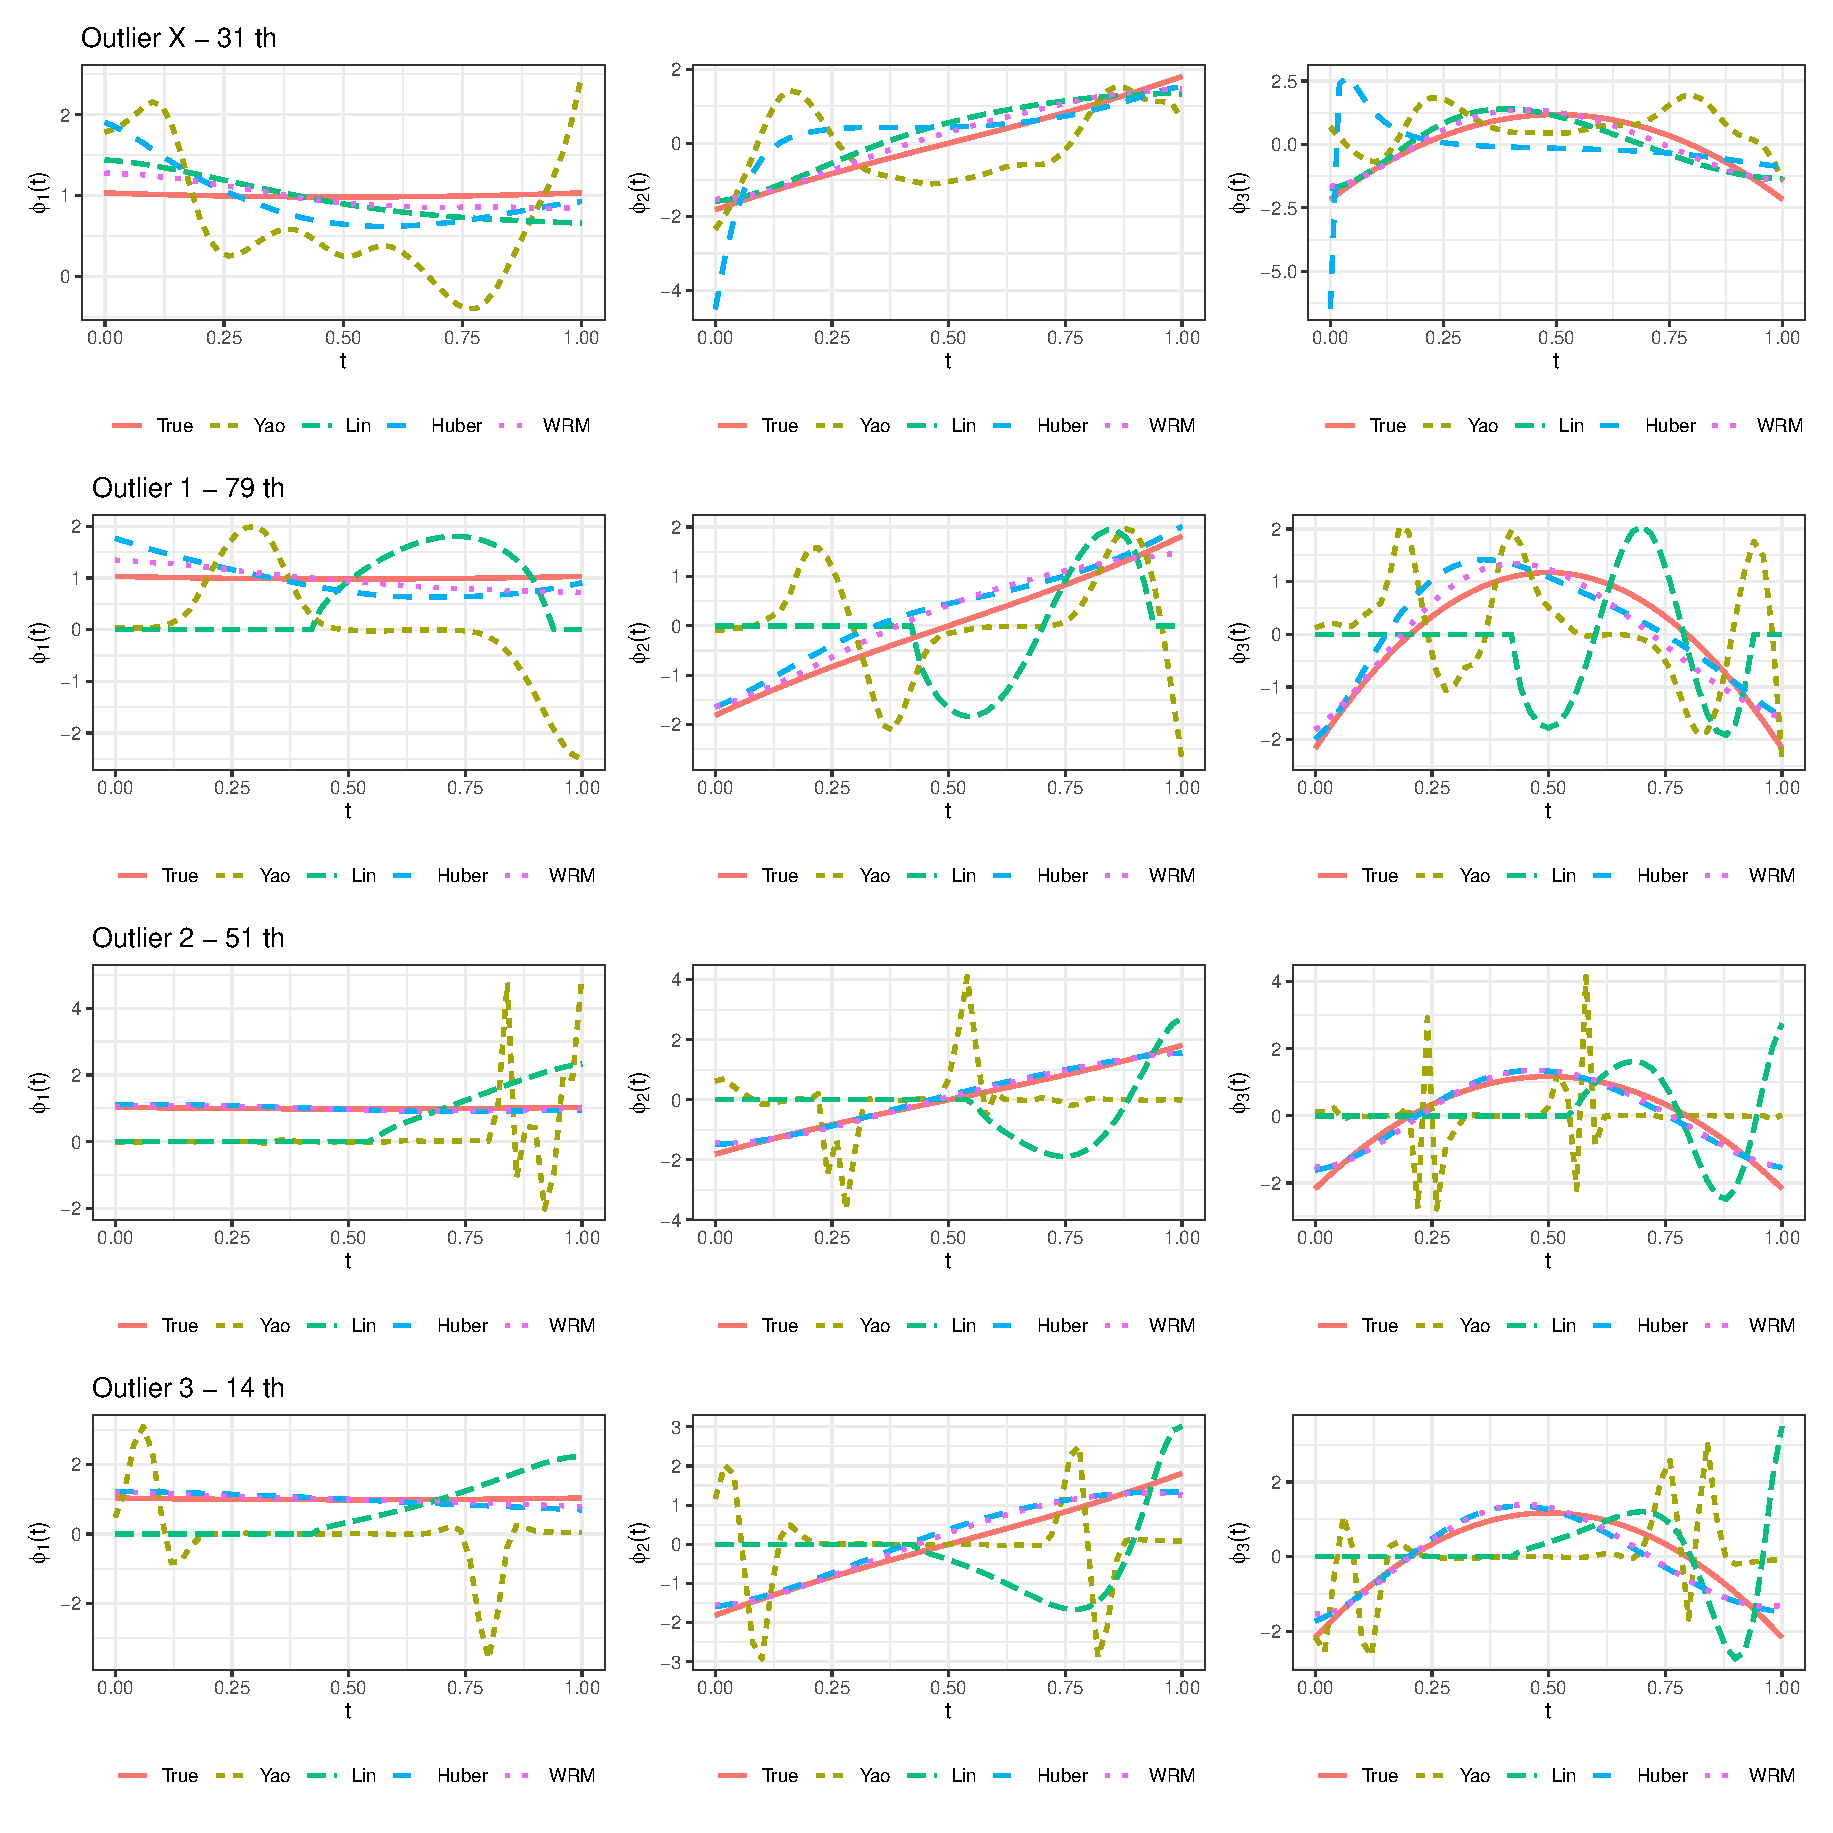
\includegraphics[height=6cm,keepaspectratio=true]{img/eig_traj.eps}
		\caption{Estimated first 3 eigenfunctions for a randomly selected simulation data.}
		\label{fig7}
	\end{figure}
\end{frame}


\begin{frame}[allowframebreaks]{Simulation results}
 	\begin{table}[ht]
 		\footnotesize
 		\centering
 		\tabcolsep=4.5pt
% 		\scriptsize
 		\begin{tabular}{cccccc}
 			\hline\hline
 			& & Yao et al. (2005) & Lin \& Wang (2020) & Huber Loss & WRM \\ 
 			\hline
 			\multirow{2}{*}{Outlier X} & $\hat{\sigma}_X^2$ & 0.93 (0.81) & 0.77 (0.44) & 1.26 (0.46) & 1.3 (0.41) \\ 
 									   & $\hat{\mathbf{C}}$ & 10.7 (237.78) & 0.61 (0.29) & 0.69 (0.20) & 0.71 (0.21) \\ 
 			\hline
 			\multirow{2}{*}{Outlier 1} & $\hat{\sigma}_X^2$ & 30.57 (3312.96) & 28.68 (2445.19) & 1.07 (0.44) & 1.12 (0.43) \\ 
 									   & $\hat{\mathbf{C}}$ & 3475.86 (104783196.62) & 14.58 (596.42) & 0.60 (0.19) & 0.60 (0.19) \\ 
 			\hline
 			\multirow{2}{*}{Outlier 2} & $\hat{\sigma}_X^2$ & 55.84 (11667.88) & 43.28 (6815.43) & 1.24 (0.45) & 1.28 (0.41) \\ 
	 		 						   & $\hat{\mathbf{C}}$ & 6029.82 (362320272.32) & 24.25 (2224.33) & 0.67 (0.19) & 0.70 (0.20) \\ 
	 		\hline
 			\multirow{2}{*}{Outlier 3} & $\hat{\sigma}_X^2$ & 700.38 (4283789.80) & 312.59 (685723.47) & 1.27 (0.46) & 1.30 (0.42) \\ 
 									   & $\hat{\mathbf{C}}$ & 27689.74 (7009102945.74) & 237.09 (435168.25) & 0.69 (0.21) & 0.70 (0.21) \\ 
 			\hline\hline
 		\end{tabular}
 		\caption{Average RMISE (standard error) of variances ($\hat\sigma^2_X$) and covariances ($\hat{\mathbf{C}}$) estimation from 100 monte carlo simulations.}\label{t1}
 	\end{table}


    \pagebreak
	\vspace*{0pt}
	\begin{table}[ht]
		\footnotesize
		\centering
		\tabcolsep=4.5pt
%		\scriptsize
		\begin{tabular}{cccccc}
			\hline\hline
			& & Yao et al. (2005) & Lin \& Wang (2020) & Huber Loss & WRM \\ 
			\hline
			\multirow{2}{*}{Outlier X} & $\mathcal{D}_0$ & 0.58 (0.28) & 0.36 (0.12) & 0.65 (0.17) & 0.66 (0.17) \\ 
									   & $\mathcal{S}_0 \backslash \mathcal{D}_0$ & 10.68 (237.77) & 0.50 (0.20) & 0.25 (0.04) & 0.25 (0.04) \\ 
			\hline
			\multirow{2}{*}{Outlier 1} & $\mathcal{D}_0$ & 35.36 (4744.87) & 13.85 (555.95) & 0.54 (0.17) & 0.55 (0.16) \\  
									   & $\mathcal{S}_0 \backslash \mathcal{D}_0$ & 3475.68 (104778703.84) & 4.56 (62.28) & 0.26 (0.06) & 0.23 (0.05) \\ 
			\hline
			\multirow{2}{*}{Outlier 2} & $\mathcal{D}_0$ & 85.62 (44631.45) & 22.71 (1936.08) & 0.63 (0.16) & 0.65 (0.17) \\ 
									   & $\mathcal{S}_0 \backslash \mathcal{D}_0$ & 6029.22 (362281921.60) & 8.49 (308.71) & 0.24 (0.04) & 0.25 (0.04) \\ 
			\hline
			\multirow{2}{*}{Outlier 3} & $\mathcal{D}_0$ & 1204.33 (13473841.14) & 193.93 (280729.87) & 0.65 (0.17) & 0.65 (0.17) \\ 
									   & $\mathcal{S}_0 \backslash \mathcal{D}_0$ & 27663.54 (6995687472.30) & 136.40 (154769.64) & 0.25 (0.04) & 0.24 (0.04) \\  
			\hline\hline
		\end{tabular}
		\caption{Average RMISE (standard error) of covariance estimation between intrapolation ($\mathcal{D}_0$) and extrapolation ($\mathcal{S}_0 \backslash \mathcal{D}_0$) parts from 100 monte carlo simulations.}\label{t2}
	\end{table}
 
 
     \pagebreak
	 \vspace*{0pt}
	 \begin{table}[ht]
	 	\footnotesize
	 	\centering
	 	\tabcolsep=4.5pt
	 	%		\scriptsize
	 	\begin{tabular}{cccccc}
	 		\hline\hline
	 		& & Yao et al. (2005) & Lin \& Wang (2020) & Huber Loss & WRM \\ 
	 		\hline
	 		\multirow{2}{*}{Outlier X} & RMISE (SE) & 2.08 (0.94) & 0.43 (0.19) & 0.64 (0.50) & 0.65 (0.64) \\ 
	 								   & PVE & 69.37 & 93.21 & 83.70 & 84.90 \\ 
	 		\hline
	 		\multirow{2}{*}{Outlier 1} & RMISE (SE) & 2.20 (0.64) & 2.00 (0.64) & 0.62 (0.40) & 0.61 (0.50) \\ 
							 		   & PVE & 66.27 & 91.75 & 83.14 & 85.63 \\ 
	 		\hline
	 		\multirow{2}{*}{Outlier 2} & RMISE (SE) & 2.13 (0.87) & 1.81 (1.42) & 0.62 (0.44) & 0.60 (0.42) \\ 
	 								   & PVE & 66.50 & 92.16 & 84.63 & 83.95 \\ 
	 		\hline
	 		\multirow{2}{*}{Outlier 3} & RMISE (SE) & 2.12 (0.67) & 1.31 (1.35) & 0.60 (0.39) & 0.59 (0.36) \\ 
	 								   & PVE & 70.28 & 94.07 & 82.95 & 84.15 \\ 
	 		\hline\hline
	 	\end{tabular}
	 	\caption{Average RMISE (standard error) of first 3 eigenfunctions and its average proportion of variance explained (PVE) from 100 monte carlo simulations.}\label{t3}
	 \end{table}
\end{frame}




%\section{Conclusion}
%
%\begin{frame}[allowframebreaks]{Conclusion}
%	\begin{itemize}
%    	\item{
%			In this study, we propose \ul{a ensemble classification method for sparse functional data}, which is a bagged model that combines classifiers based on FPC scores.
%		}
%	\end{itemize}
%\end{frame}



\section*{Reference}
\begin{frame}[allowframebreaks]
	\frametitle<presentation>{Reference}
	\renewcommand{\section}[2]{}   % delete "References" section title
	\begin{thebibliography}{9}
		\footnotesize
        
        \bibitem[{Fried et~al.(2007)}]{Fried2007}
        Fried, R., Einbeck, J., \& Gather, U. (2007). Weighted repeated median smoothing and filtering. {\em Journal of the American Statistical Association}, 102(480), 1300-1308.
        
        \bibitem[{Huber(1964)}]{Huber1964}
        Huber, P. J. (1964). Robust Estimation of a Location Parameter. {\em The Annals of Mathematical Statistics}, 73-101.
        
        \bibitem[{Kraus(2015)}]{Kraus2015}
        Kraus, D. (2015). Components and completion of partially observed functional data. {\em Journal of the Royal Statistical Society: Series B: Statistical Methodology}, 777-801.
        
        \bibitem[{Lin and Wang(2020)}]{Lin2020}
        Lin, Z., \& Wang, J. L. (2020). Mean and covariance estimation for functional snippets. {\em Journal of the American Statistical Association}, 1-13.
        
        \bibitem[{Yao et~al.(2005)}]{Yao2005}
        Yao, F., Müller, H. G., \& Wang, J. L. (2005). Functional data analysis for sparse longitudinal data. {\em Journal of the American Statistical Association}, {\bf 100}, 577-590.
	\end{thebibliography}	
\end{frame}


\begin{frame}
	\begin{center}
		\huge
		\textbf{Thank You!}
	\end{center}
\end{frame}


\end{document}


